\documentclass[12pt]{report}

% -------------------------------------------------
% PACKAGES
% -------------------------------------------------
\usepackage[a4paper,margin=1in]{geometry}
\usepackage{graphicx}
\usepackage{setspace}
\usepackage{titlesec}
\usepackage{tocloft}
\usepackage{amsmath}
\usepackage{booktabs}
\usepackage{float}

\setstretch{1.2}

% -------------------------------------------------
% DOCUMENT
% -------------------------------------------------
\begin{document}

% =================================================
% TITLE PAGE
% =================================================
\begin{titlepage}

\begin{center}

\vspace*{1cm}

{\Large \textbf{Energy-Aware Online Positioning of UAV Base Stations in Dynamic Networks}}

\vspace{1cm}

A Project Report submitted in partial fulfillment of the requirements for the award of the degree of

\vspace{1cm}

{\large \textbf{Bachelor of Technology}}

\vspace{0.3cm}

in

\vspace{0.3cm}

{\large \textbf{Electronics and Communication Engineering}}

\vspace{1cm}

by

\vspace{0.5cm}

\textbf{
Nikhil (112316031) \\
Visweswar (112316009) \\
Vinit (112316010) \\
Sangamesh (112316041) \\
Bhavya (112316012)
}

\vspace{1cm}

Under the Supervision of: \textbf{Supervisor's Name}

\vspace{1cm}

\textbf{Semester: VI}

\vspace{1cm}

% -------------------------------------------------
% LOGO
% -------------------------------------------------

\includegraphics[width=0.25\textwidth]{logo.png}

\vfill

\textbf{
Department of Electronics and Communication Engineering
}

\vspace{0.5cm}

\textbf{
Indian Institute of Information Technology, Pune
}

\vspace{0.3cm}

(An Institute of National Importance)

\vspace{1cm}

\textbf{MAY 2026}

\end{center}

\end{titlepage}

% =================================================
% INDEX
% =================================================
\tableofcontents
\newpage

% =================================================
% INTRODUCTION
% =================================================

\chapter{Introduction}

\section{Background}

Wireless cellular networks are designed to provide reliable coverage and sufficient traffic handling capacity under normal operating conditions. However, during emergency situations such as natural disasters, infrastructure failures, or large-scale public events, parts of the network may become overloaded or completely non-operational. In such scenarios, conventional terrestrial base stations may not provide adequate connectivity, leading to coverage gaps and a poor quality of service for users.

To address these challenges, UAV-mounted base stations have emerged as a flexible and rapidly deployable solution. UAV-based base stations can dynamically provide temporary wireless coverage in affected areas and assist overloaded regions experiencing sudden traffic demand. Their mobility allows them to reposition themselves according to changing network conditions, making them highly suitable for emergency communication systems and dynamic wireless environments.

The effectiveness of UAV-assisted communication systems strongly depends on the positioning of the drone-mounted base station. A well-positioned UAV can significantly improve network performance by extending coverage, reducing interference, and supporting users that would otherwise remain unserved. Conversely, poor positioning may lead to inefficient coverage and increased interference with operational terrestrial base stations. Determining an appropriate UAV position is therefore a critical problem in dynamic wireless networks.

Furthermore, the positioning problem becomes increasingly challenging due to factors such as unknown user distribution, changing traffic hotspots, varying propagation conditions, and the trade-off between coverage restoration and capacity enhancement. As a result, several recent works have focused on proposing various methods to solve this positioning problem

\section{Motivation}

Online UAV positioning approaches have demonstrated significant improvements in network performance by dynamically adapting the drone location according to changing wireless conditions. These methods are capable of improving coverage and maintaining communication quality during network disruptions and traffic hotspot scenarios.

However, most existing approaches primarily focus on optimizing communication-centric metrics such as coverage, throughput, and Call Success Rate (CSR), while neglecting the practical energy limitations of UAV systems. In many cases, the UAV continuously repositions itself to achieve marginal performance improvements, resulting in excessive movement and increased propulsion energy consumption.

Since UAVs are inherently battery-constrained systems, frequent movement can significantly reduce operational lifetime and limit the practicality of real-time deployment. This motivates the need for an energy-aware positioning framework capable of balancing communication performance with movement energy cost while still maintaining reliable wireless service.
% =================================================
% LITERATURE REVIEW
% =================================================
\chapter{Literature Review}

\section{Base Paper Overview}

The primary reference for this work is the paper titled \textit{“Online Positioning of a Drone-Mounted Base Station in Emergency Scenarios”}. :contentReference[oaicite:0]{index=0} The paper proposes a real-time, data-driven positioning algorithm for UAV-mounted base stations operating in emergency communication scenarios such as natural disasters, infrastructure failures, and sudden traffic hotspot events.

The base paper addresses the problem of dynamically positioning a drone-mounted base station in order to restore wireless coverage and improve network capacity when terrestrial infrastructure becomes unavailable or overloaded. Unlike conventional optimization approaches that require complete environmental knowledge or offline training, the proposed method operates online using real-time network measurements.

The authors analyze several control parameters including UAV horizontal position, altitude, and Cell Individual Offset (CIO). Through simulation-based sensitivity analysis, the study concludes that horizontal positioning has the greatest impact on network performance, while altitude and CIO have comparatively smaller influence on the Call Success Rate (CSR). As a result, the proposed online algorithm primarily adjusts the UAV’s horizontal position.

A major contribution of the base paper is the evaluation of multiple control metrics for UAV movement decisions. Among the evaluated metrics, the metric referred to as \textbf{CM7} was found to have the strongest correlation with CSR performance. CM7 represents the average load per user across the drone cell and the most heavily loaded neighboring cell. Using this metric, the UAV continuously adjusts its position toward regions that improve network performance.

The paper demonstrates that online UAV positioning significantly improves communication performance compared to static deployment strategies. It also shows that the algorithm can dynamically adapt to moving traffic hotspots and changing user distributions without requiring prior knowledge of the environment. However, the positioning decisions are primarily focused on communication performance and do not explicitly account for UAV propulsion energy consumption. :contentReference[oaicite:1]{index=1}

\section{Related Research}

Several research works have explored UAV-assisted wireless communication systems, focusing on positioning optimization, coverage enhancement, and energy efficiency.

One important supporting work is \textit{“Energy-aware Relay Positioning in Flying Networks”}. :contentReference[oaicite:2]{index=2} This paper studies the positioning of Flying Communication Relay (FCR) UAVs while considering propulsion energy consumption. The authors highlight that UAV propulsion energy dominates communication energy consumption and demonstrate that hovering is not always the most energy-efficient operating state.

The paper proposes the \textbf{Energy-aware Relay Positioning (EREP)} algorithm, which determines UAV trajectories and movement speeds that minimize propulsion energy while maintaining communication quality. The work models propulsion power using blade profile, induced, and parasite power components. Simulation results show significant improvements in UAV endurance with only negligible degradation in throughput and delay performance. However, the proposed framework assumes a controlled network topology and relies on predefined environmental information, making it less suitable for lightweight real-time adaptive deployment scenarios. :contentReference[oaicite:3]{index=3}

Another relevant direction in the literature involves reinforcement learning-based UAV positioning approaches. Methods such as \textit{Efficient 3D Aerial Base Station Placement Considering Users Mobility by Reinforcement Learning} employ machine learning algorithms to dynamically optimize UAV placement under changing user mobility conditions. These approaches can adapt to complex environments and varying traffic distributions. However, they typically require extensive training data, high computational resources, and long convergence times, which may limit their applicability in emergency communication scenarios requiring rapid deployment.

In addition, survey papers on UAV-assisted wireless communication systems provide comprehensive overviews of UAV deployment architectures, air-to-ground propagation models, positioning strategies, energy constraints, and mobility management challenges. These studies emphasize that UAV positioning is influenced by multiple interacting factors including coverage requirements, user distribution, interference, battery limitations, and dynamic traffic conditions. They further identify energy efficiency and real-time adaptability as key research challenges in practical UAV communication systems.

Collectively, existing literature demonstrates that UAV-mounted base stations can significantly improve wireless communication performance in dynamic and emergency environments. However, many existing solutions either focus solely on communication performance or rely on computationally intensive optimization methods that are difficult to implement in practical real-time systems.

\section{Existing Challenges}

Despite significant advancements in UAV-assisted wireless communication systems, several important challenges still remain unresolved.

A major limitation of many existing online UAV positioning algorithms is that they primarily optimize communication-centric metrics such as throughput, coverage probability, spectral efficiency, or Call Success Rate (CSR), while neglecting the propulsion energy consumed by UAV movement. Since UAVs are battery-constrained systems, continuous repositioning can rapidly deplete onboard energy and reduce operational lifetime.

Another challenge arises from the dynamic nature of wireless environments. User distributions, traffic hotspots, and interference conditions may continuously change over time. Therefore, UAV positioning algorithms must rapidly adapt to changing network conditions without relying on prior environmental knowledge or offline optimization.

Several machine learning and reinforcement learning-based positioning approaches have been proposed to address environmental uncertainty. However, these methods often require large training datasets, high computational complexity, and long convergence periods, making them less practical for emergency deployment scenarios where rapid response is critical.

Energy-aware positioning methods such as EREP successfully incorporate propulsion energy models into UAV movement decisions. However, these approaches generally assume controlled network topology, known system parameters, or predefined trajectories, which limits their ability to operate in fully online and dynamic environments.

Furthermore, there exists an important trade-off between communication performance and energy efficiency. Aggressive UAV movement may slightly improve network performance but can substantially increase propulsion energy consumption. Conversely, minimizing movement excessively may degrade coverage and CSR performance. Designing a lightweight real-time positioning framework capable of balancing this trade-off remains an open research problem.

Therefore, there is a clear need for an energy-aware online UAV positioning framework that can dynamically adapt to changing wireless conditions while simultaneously considering both communication performance and UAV energy consumption. The proposed work aims to address this research gap by integrating movement energy cost into the real-time UAV positioning decision process using a lightweight control metric-based approach. :contentReference[oaicite:4]{index=4} :contentReference[oaicite:5]{index=5}

% =================================================
% PROBLEM STATEMENT
% =================================================
% =================================================
% PROBLEM STATEMENT AND RESEARCH GAP
% =================================================

\chapter{Problem Statement and Research Gap}

\section{Problem Statement}

In dynamic wireless communication scenarios such as emergency response situations and traffic hotspot events, UAV-mounted base stations are deployed to provide temporary coverage and capacity enhancement. Existing online positioning algorithms dynamically reposition the UAV to maximize communication performance metrics such as coverage and Call Success Rate (CSR). However, these approaches often result in continuous UAV movement in pursuit of marginal performance improvements.

Since UAVs are battery-constrained systems, frequent repositioning introduces significant propulsion energy consumption and reduces operational efficiency. Therefore, there exists a need for a positioning mechanism that can balance communication performance with the energy cost associated with UAV movement.

\section{Research Gap}

Several existing works have proposed adaptive UAV positioning techniques for wireless communication systems. Most of these approaches focus primarily on optimizing network-centric metrics such as coverage probability, throughput, and CSR, while assuming unlimited UAV energy availability. As a result, the movement cost of the UAV is often neglected during positioning decisions.

Although some energy-aware UAV positioning approaches exist as discussed in the previous section, many of them rely on prior environmental knowledge, offline optimization, or computationally expensive learning-based methods that are less suitable for lightweight real-time deployment.

Therefore, a practical research gap exists in developing a real-time, energy-aware UAV positioning framework that can dynamically adapt to changing network conditions while incorporating movement energy constraints into the positioning decision process.

\section{Objectives}

The primary objective of this work is to develop and evaluate an energy-aware online UAV positioning framework for dynamic wireless communication scenarios involving network failures and traffic hotspots.

The specific objectives of the proposed work are as follows:

\begin{itemize}
    \item To study and analyze existing online UAV positioning technique used for emergency wireless communication systems.
    
    \item To evaluate the performance of different control metrics for adaptive UAV positioning across urban and rural deployment scenarios.
    
    \item To incorporate movement energy cost into the UAV positioning decision process in order to reduce unnecessary UAV repositioning.
    
    \item To analyze the trade-off between UAV movement reduction and Call Success Rate (CSR) performance under varying network conditions.
    
\end{itemize}
% =================================================
% SYSTEM MODEL
% =================================================

\chapter{System Model}

\section{Network Architecture}

The simulated wireless communication system consists of a hexagonal cellular network containing 12 three-sectorized base station sites, resulting in a total of 36 cells. To reduce edge effects and emulate a large-scale deployment environment, the network employs wraparound boundary conditions.

Under normal operating conditions, all terrestrial base stations remain active and provide wireless connectivity to users distributed across the network area. To model an emergency communication scenario, one base station site is assumed to fail, creating a coverage hole and reduced service availability in the affected region. A UAV-mounted base station is subsequently deployed to provide temporary coverage assistance and improve network performance.

The UAV functions as a mobile aerial base station operating at a fixed altitude. It dynamically repositions itself in the horizontal plane according to the positioning algorithm in order to adapt to changing network conditions. Both urban and rural deployment environments are considered to evaluate system behavior under different propagation and traffic characteristics.

The network additionally includes traffic hotspot regions with increased user density and communication demand. These hotspots represent realistic situations such as emergency response areas, crowded public events, or disaster-affected zones where temporary network congestion may occur.

\section{Communication Model}

The communication framework considers both terrestrial and air-to-ground wireless links. Communication between terrestrial base stations and user equipment follows conventional cellular propagation behavior, while communication between the UAV and users is modeled using an air-to-ground propagation model incorporating both Line-of-Sight (LoS) and Non-Line-of-Sight (NLoS) conditions.

The probability of LoS communication depends on the elevation angle between the UAV and the user equipment. Path loss calculations further incorporate shadow fading effects and minimum coupling loss in order to model realistic wireless channel conditions.

Users are associated with the cell providing the strongest received signal strength. The system additionally incorporates admission control, resource allocation, and handover mechanisms to dynamically manage network resources under changing traffic conditions.

\section{Performance Metrics}

The primary performance metric used in this work is the Call Success Rate (CSR), defined as the fraction of user calls that are successfully admitted and maintained while satisfying the minimum communication requirements.

To evaluate the efficiency of the proposed positioning approach, UAV movement behavior is also analyzed. The total number of movement steps performed by the UAV is used as an approximate indicator of propulsion energy consumption. A reduction in unnecessary movement corresponds to improved energy efficiency and enhanced operational stability.

The proposed energy-aware positioning framework is compared against the baseline online positioning method in terms of both communication performance and movement efficiency.

\section{Modeling Assumptions}

Several assumptions are adopted in order to simplify the simulation environment while preserving realistic system behavior. The UAV operates at a fixed altitude throughout the simulation and moves only in the horizontal plane using discrete movement steps determined by the positioning algorithm. User equipment remains static during active communication sessions.

A simplified discrete energy model is employed in which UAV movement and hovering consume fixed energy values per simulation step. The model primarily focuses on propulsion-related energy consumption and does not explicitly consider aerodynamic effects, acceleration dynamics, or communication hardware power consumption.

The simulations are conducted under both urban and rural deployment scenarios using predefined propagation parameters, hotspot configurations, and traffic generation models. Multiple simulation runs are averaged to reduce randomness and improve the consistency of the observed results.
% =================================================
% PROPOSED METHOD
% =================================================
% =================================================
% PROPOSED ENERGY-AWARE IMPROVEMENT
% =================================================

\chapter{Proposed Energy-Aware Improvement}

\section{Baseline Positioning Method}

The baseline positioning approach is based on the online drone positioning algorithm proposed in the reference paper. The algorithm dynamically adjusts the horizontal position of the UAV-mounted base station using real-time network measurements in order to improve communication performance during emergency scenarios.

The original framework operates by iteratively moving the UAV in the horizontal plane and evaluating the effect of each movement using a control metric (CM). The UAV continuously adjusts its position in the direction that improves the selected control metric, allowing the drone to adapt to changing user distributions and traffic hotspot conditions without requiring prior environmental knowledge or offline training.

Among the evaluated control metrics, the CM7 metric was identified as the most effective for approximating the Call Success Rate (CSR). CM7 represents the average load per user across the drone cell and the most heavily loaded neighboring cell, weighted according to the number of users served by each cell.

Although the baseline approach achieves strong communication performance, it continuously repositions the UAV in pursuit of small performance gains. As a result, the algorithm does not consider the propulsion energy consumed during movement and implicitly assumes unlimited UAV battery capacity.

\section{Energy Consumption Model}

To incorporate energy awareness into the positioning process, a simplified discrete energy model is introduced. The model approximates propulsion-related energy consumption using fixed energy costs associated with UAV movement and hovering operations.

At each simulation step, the UAV consumes:
\[
E =
\begin{cases}
\alpha, & \text{if the UAV moves} \\
\beta, & \text{if the UAV hovers}
\end{cases}
\]

where:
\begin{itemize}
    \item $\alpha$ represents the energy cost of a movement step,
    \item $\beta$ represents the energy cost during hovering.
\end{itemize}

The model is intentionally simplified in order to support lightweight real-time decision making without requiring complex aerodynamic or mechanical calculations. Although the model does not explicitly consider velocity variation, acceleration, or communication hardware power consumption, it effectively captures the relative energy cost associated with unnecessary UAV movement.

\section{Proposed Algorithm}

The proposed approach extends the baseline online positioning framework by introducing energy-aware decision making into the movement process. Instead of moving solely to maximize communication performance, the UAV evaluates whether the expected performance improvement justifies the corresponding movement energy cost.

The algorithm continues to use the CM7 control metric as the primary indicator of network performance. At each decision step, the UAV measures the change in the control metric after movement and computes the corresponding performance gain.

The gain is defined as:
\[
\text{Gain} = CM7_{old} - CM7_{new}
\]

A movement is accepted only when:
\[
\text{Gain} > \lambda \times \text{Energy} + \epsilon
\]

where:
\begin{itemize}
    \item $\lambda$ is the trade-off parameter controlling the balance between performance and energy efficiency,
    \item $\epsilon$ is a small threshold used to prevent unnecessary movement caused by minor fluctuations or measurement noise.
\end{itemize}

If the observed improvement is insufficient, the UAV avoids unnecessary repositioning and either remains stationary or explores an alternative direction. This allows the drone to stabilize near efficient operating positions instead of continuously chasing marginal performance improvements.

\section{Algorithm Workflow}

Figure X illustrates the workflow of the proposed energy-aware positioning algorithm. The UAV continuously evaluates the CM7 control metric and compares the observed performance improvement against the estimated movement energy cost. Based on this comparison, the UAV either continues movement in the current direction or stabilizes to avoid unnecessary energy expenditure.

\begin{figure}[H]
    \centering
    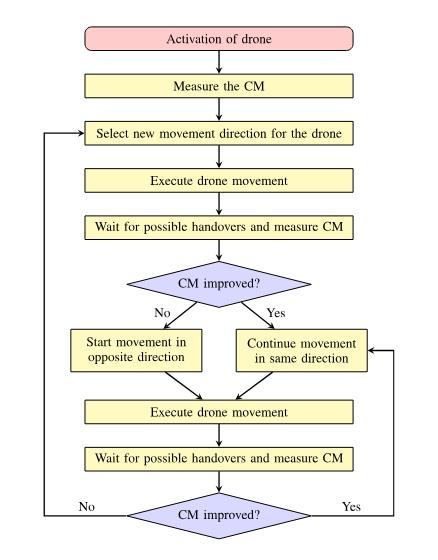
\includegraphics[width=0.75\textwidth]{workflow.png}
    \caption{Workflow of the proposed energy-aware UAV positioning algorithm}
    \label{fig:workflow}
\end{figure}% =================================================
% SIMULATION SETUP
% =================================================
% =================================================
% SIMULATION SETUP
% =================================================

\chapter{Simulation Setup}

\section{Simulation Environment}

The proposed UAV positioning framework is evaluated using a large-scale wireless cellular network simulation modeled according to the reference system described in the base paper. The simulated network consists of 12 three-sectorized base station sites, resulting in a total of 36 cells. Wraparound boundary conditions are employed to reduce edge effects and emulate a continuous deployment environment.

The simulation models an emergency communication scenario in which one terrestrial base station site fails, creating a coverage hole within the network. Following the failure event, a UAV-mounted base station is deployed to provide temporary coverage support and dynamically reposition itself according to the selected positioning algorithm.

Both urban and rural deployment environments are considered during evaluation. These environments differ in terms of inter-site distance, propagation characteristics, hotspot intensity, and traffic load. The urban environment represents dense deployments with higher traffic concentration and stronger interference effects, while the rural environment models wider coverage areas with comparatively lower user density.

Traffic hotspot regions are additionally introduced to simulate areas of concentrated communication demand. These hotspots represent realistic scenarios such as disaster response regions, crowded public events, or temporary traffic surges.

The simulation process consists of multiple operational phases. Initially, the network operates under normal conditions in order to establish stable traffic behavior. A base station failure is then introduced, after which the UAV is activated and begins dynamic positioning using either the baseline or the proposed energy-aware positioning algorithm.

\section{Simulation Parameters}

The simulation parameters are primarily derived from the reference paper and adapted for the proposed energy-aware positioning framework. The UAV operates at a fixed altitude and performs discrete horizontal movement steps during online positioning. Real-time control decisions are evaluated periodically using the CM7 control metric.

Table~\ref{tab:simparams} summarizes the key simulation parameters used throughout the evaluation.

\begin{table}[H]
\centering
\caption{Simulation Parameters}
\label{tab:simparams}
\begin{tabular}{|l|c|}
\hline
\textbf{Parameter} & \textbf{Value} \\ \hline

Number of Sites & 12 \\ \hline
Number of Cells & 36 \\ \hline
Carrier Frequency & 3.5 GHz \\ \hline
Bandwidth per Cell & 5 MHz \\ \hline
Urban ISD & 500 m \\ \hline
Rural ISD & 3500 m \\ \hline
UAV Altitude & 120 m \\ \hline
Drone Step Size & 1 m \\ \hline
Drone Speed & 24 km/h \\ \hline
Measurement Period & 200 ms \\ \hline
Control Interval & 400 ms \\ \hline
Coverage Threshold & -120 dBm \\ \hline
Minimum Bitrate Requirement & 0.384 Mbps \\ \hline
Average Call Duration & 120 s \\ \hline
Hotspot Radius & 100 m \\ \hline
Simulation Runs & 25 \\ \hline
Energy Cost Parameter ($Energy$) & 0.01 \\ \hline
Weighting Factor ($\alpha$) & 1.3 \\ \hline
Threshold Parameter ($\epsilon$) & 0.001 \\ \hline

\end{tabular}
\end{table}

The urban deployment scenarios use hotspot intensity multipliers of 2, 4, and 8, while the rural scenarios use multipliers of 10, 25, and 50 in order to model varying traffic congestion conditions. Multiple simulation runs are averaged to reduce randomness and improve result consistency. :contentReference[oaicite:0]{index=0}

\section{Evaluation Criteria}

The performance of the proposed energy-aware positioning framework is evaluated by comparing it against the baseline online UAV positioning algorithm under identical network conditions.

The primary evaluation metric used in this work is the Call Success Rate (CSR), which represents the fraction of user calls successfully admitted and maintained while satisfying the minimum communication requirements. CSR is used to evaluate the overall communication effectiveness of the positioning strategy under different deployment scenarios.

In addition to communication performance, UAV movement behavior is also analyzed in order to evaluate operational efficiency. The total number of movement steps performed by the UAV is used as an approximate indicator of propulsion-related energy consumption. Lower movement counts correspond to reduced energy expenditure and improved deployment stability.

Performance comparisons are conducted across multiple urban and rural deployment scenarios with varying hotspot intensities and failure conditions. The evaluation includes comparisons between:
\begin{itemize}
    \item No-drone deployment scenarios,
    \item Static UAV deployment,
    \item Baseline online positioning methods using different control metrics,
    \item The proposed energy-aware CM7 positioning framework.
\end{itemize}

The analysis further considers convergence behavior, communication stability, and the trade-off between communication performance and movement efficiency across different network environments.
% =================================================
% PERFORMANCE EVALUATION, RESULTS, AND DISCUSSION
% =================================================

\chapter{Performance Evaluation, Results, and Discussion}

This chapter presents the experimental evaluation of the proposed energy-aware UAV positioning framework. The analysis is organized into three primary stages. First, the effectiveness of the different control metrics used for online UAV positioning is evaluated across urban and rural deployment scenarios. Next, the temporal convergence behavior of the positioning framework is analyzed in order to study operational stability after UAV deployment. Finally, the energy-aware positioning strategy is evaluated in terms of the trade-off between communication performance and UAV movement efficiency.

% =================================================
\section{Control Metric Evaluation}

The first stage of evaluation focuses on comparing the performance of the different control metrics used for online UAV positioning. The evaluated methods are compared against two reference deployment configurations:
\begin{itemize}
    \item No-drone deployment,
    \item Static drone deployment.
\end{itemize}

The comparison is performed across multiple urban (DU) and rural (RU) deployment scenarios with varying hotspot intensities and failure conditions.

Figures~\ref{fig:du_heatmap} and~\ref{fig:ru_heatmap} illustrate the normalized performance of the evaluated positioning methods across urban and rural deployment scenarios, respectively.

\begin{figure}[H]
    \centering
    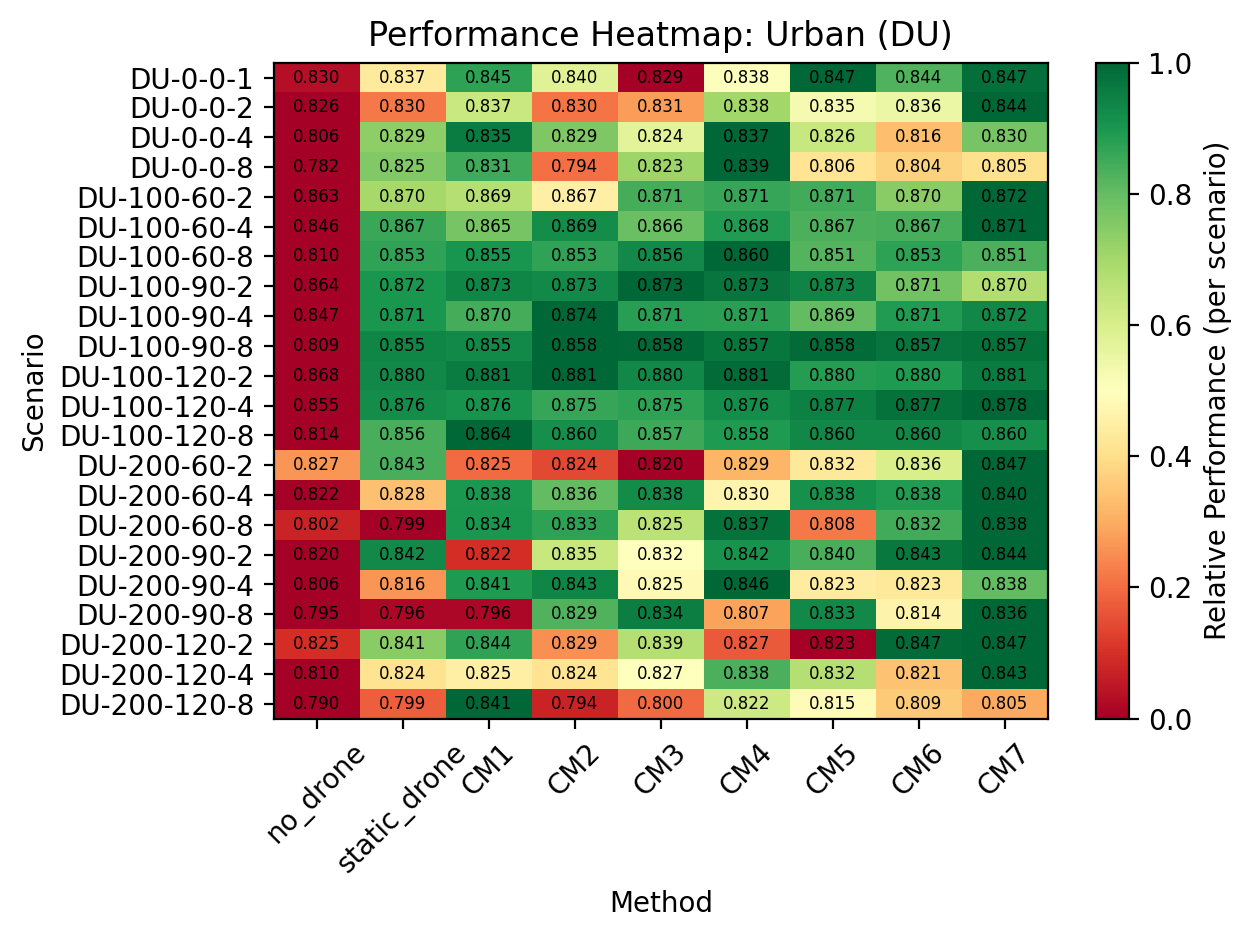
\includegraphics[width=0.9\textwidth]{performance_heatmap_DU.png}
    \caption{Performance comparison of control metrics across urban deployment scenarios}
    \label{fig:du_heatmap}
\end{figure}

\begin{figure}[H]
    \centering
    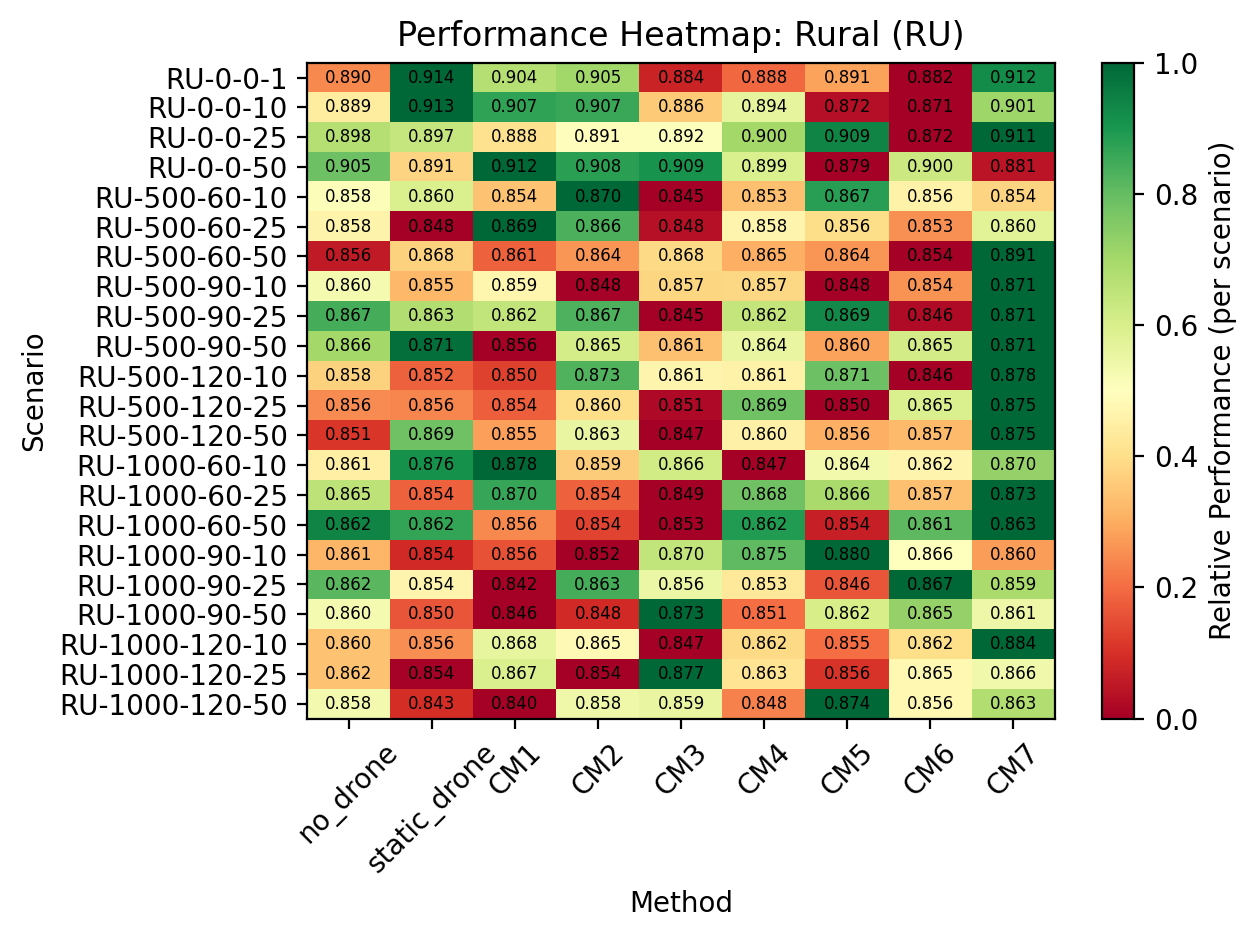
\includegraphics[width=0.9\textwidth]{performance_heatmap_RU.png}
    \caption{Performance comparison of control metrics across rural deployment scenarios}
    \label{fig:ru_heatmap}
\end{figure}

The results demonstrate that dynamic UAV positioning consistently improves network performance compared to both the no-drone and static-drone configurations. The performance improvement is especially visible in scenarios with severe traffic hotspots and larger coverage disruptions, where adaptive UAV repositioning allows the network to better respond to changing user demand.

Among the evaluated control metrics, CM7 demonstrates the most stable and consistently strong performance across both urban and rural deployment environments. Metrics such as CM1 and CM2 perform adequately under moderate traffic conditions but exhibit larger fluctuations under highly congested scenarios. CM7 achieves a more balanced distribution between drone load and neighboring cell load, enabling improved Call Success Rate (CSR) performance under varying network conditions.

Figure~\ref{fig:bar_comparison} further compares the CSR performance of the no-drone, static-drone, and CM7-based positioning approaches for individual deployment scenarios.

\begin{figure}[H]
    \centering
    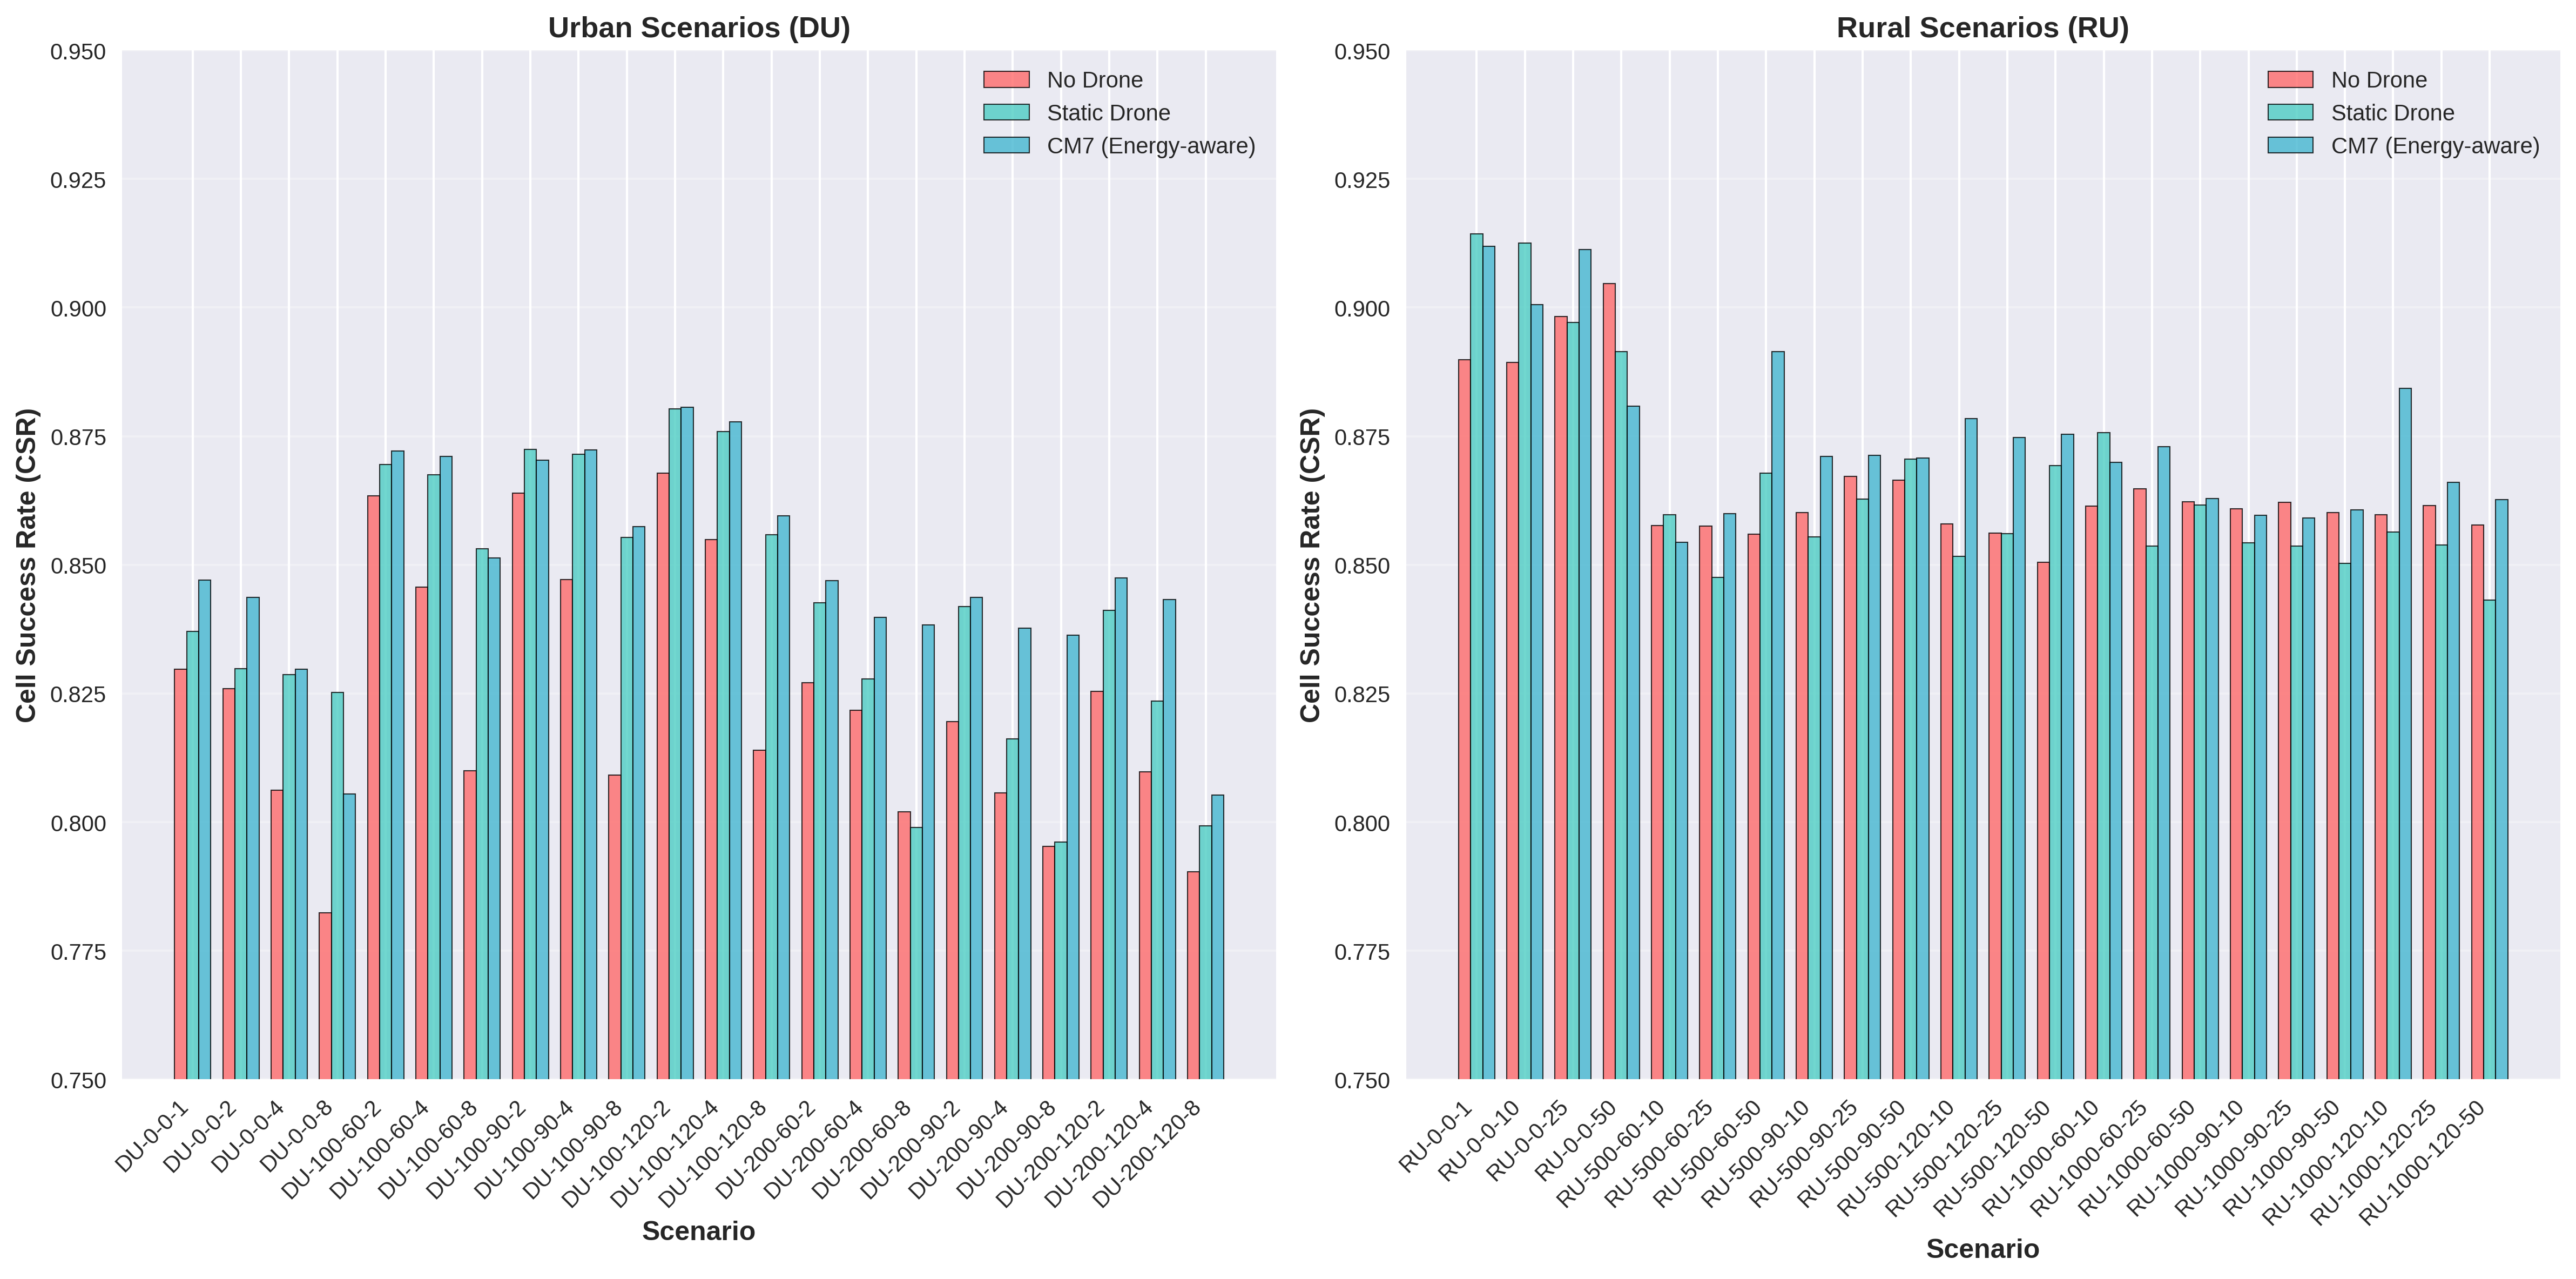
\includegraphics[width=\textwidth]{algorithm_comparison_split.png}
    \caption{CSR comparison across urban and rural deployment scenarios}
    \label{fig:bar_comparison}
\end{figure}

The grouped comparison confirms that the CM7-based positioning framework consistently achieves higher CSR values than the no-drone and static-drone configurations across most scenarios. The improvement is particularly noticeable in urban hotspot environments where adaptive repositioning enables stronger load balancing and more efficient user coverage.

The results additionally indicate that rural deployment scenarios generally achieve higher absolute CSR values than urban environments. This behavior is primarily caused by lower interference levels and wider spatial user distribution in rural networks. In contrast, urban scenarios exhibit stronger performance variation due to higher traffic density and increased inter-cell interference.

Overall, the control metric evaluation establishes CM7 as the most effective and stable metric for online UAV positioning across varying deployment conditions. Consequently, CM7 is selected as the primary control metric for the proposed energy-aware positioning framework.

% =================================================
\section{Temporal Convergence Behavior}

The second stage of evaluation analyzes the convergence characteristics of the UAV positioning framework by observing the variation of CSR over time following UAV deployment. This analysis is performed in order to study the operational stability of the positioning algorithm under representative urban and rural deployment scenarios.

Figure~\ref{fig:convergence} illustrates the convergence behavior of multiple deployment scenarios aligned at the time of UAV activation.

\begin{figure}[H]
    \centering
    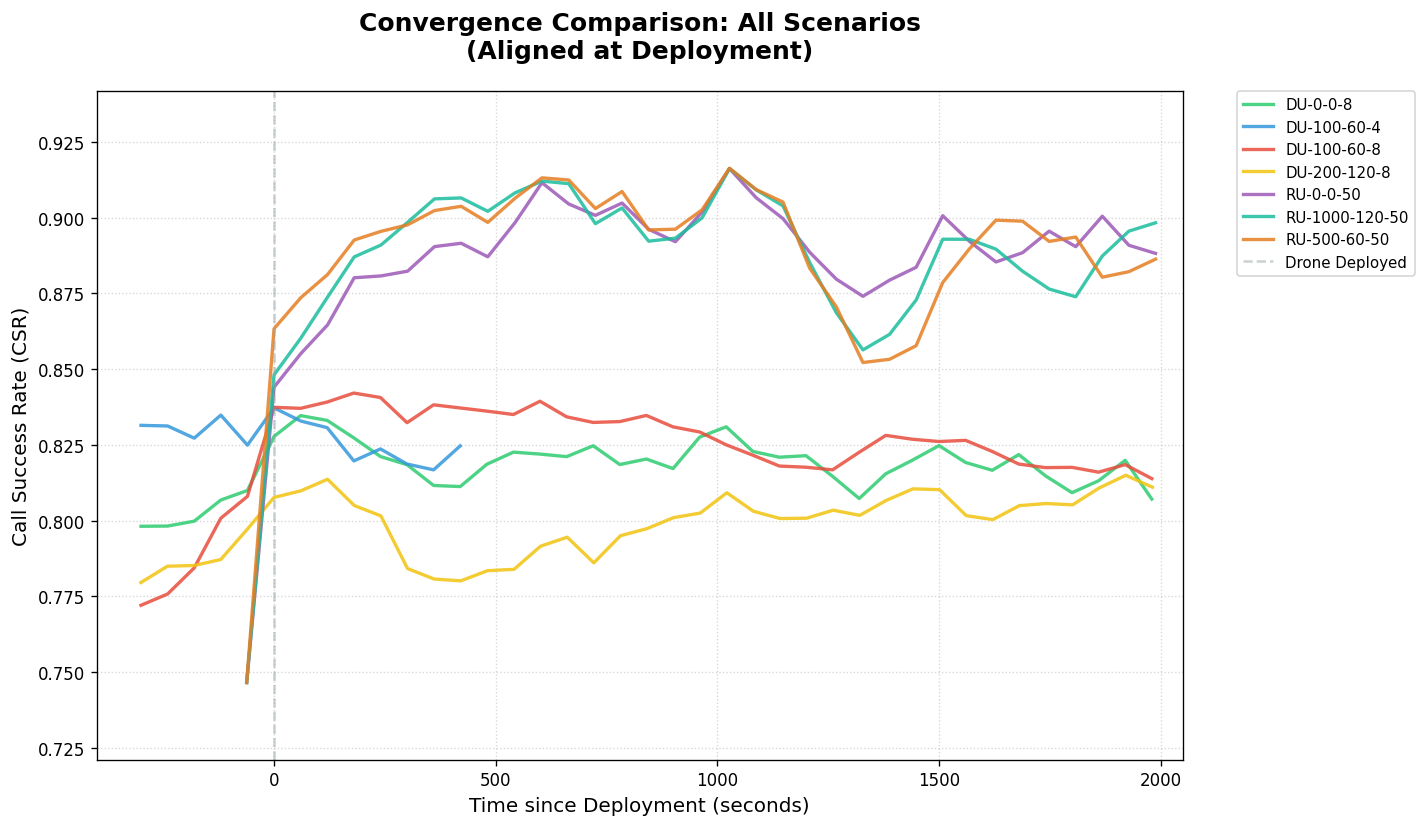
\includegraphics[width=\textwidth]{convergence_comparison_all.png}
    \caption{Convergence behavior of the UAV positioning framework across multiple deployment scenarios}
    \label{fig:convergence}
\end{figure}

The results show that UAV deployment immediately improves communication performance following the occurrence of a site failure. In several scenarios, CSR increases rapidly after deployment and gradually stabilizes near a steady operating point as the UAV adapts to changing network conditions.

The convergence curves further demonstrate that the positioning framework maintains relatively stable CSR values after the initial adaptation phase. Although temporary fluctuations occur due to changing hotspot intensity and network load distribution, the algorithm successfully avoids large oscillatory behavior and converges toward stable operating conditions.

Urban deployment scenarios generally exhibit greater CSR variability due to stronger interference effects and higher traffic concentration. Rural scenarios, on the other hand, display comparatively smoother convergence behavior because of lower interference and more stable user distribution patterns.

The convergence analysis therefore indicates that the proposed positioning framework is capable of adapting dynamically to changing wireless conditions while maintaining stable long-term communication performance.

% =================================================
\section{Energy-Aware Positioning Trade-off}

The final stage of evaluation analyzes the effectiveness of the proposed energy-aware positioning strategy in reducing unnecessary UAV movement while preserving communication performance.

Figure~\ref{fig:tradeoff} presents the relationship between the number of movement steps saved relative to the legacy positioning algorithm and the corresponding CSR difference between the energy-aware and legacy approaches.

\begin{figure}[H]
    \centering
    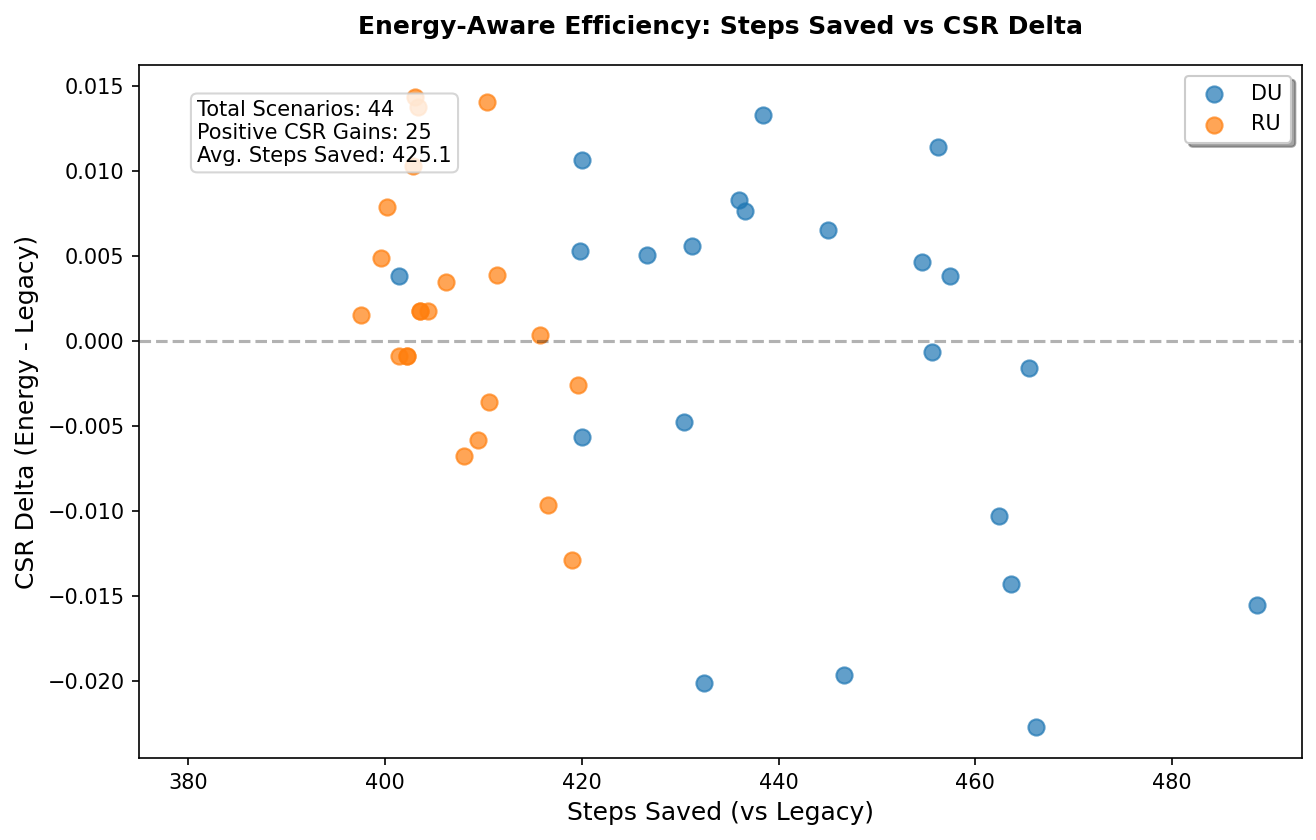
\includegraphics[width=0.85\textwidth]{energy_tradeoff_analysis.png}
    \caption{Movement efficiency versus CSR difference for the proposed energy-aware positioning framework}
    \label{fig:tradeoff}
\end{figure}

The results indicate that the proposed energy-aware framework achieves substantial reductions in UAV movement across nearly all evaluated scenarios. On average, more than 400 movement steps are eliminated relative to the legacy positioning approach, significantly reducing propulsion-related energy expenditure.

At the same time, the observed CSR variation remains relatively small across most deployment scenarios. Several cases even demonstrate slight CSR improvements despite the reduction in movement, indicating that continuous repositioning is not always necessary for maintaining effective communication performance.

The analysis additionally reveals a clear trade-off between communication performance and movement efficiency. While a limited number of scenarios experience minor CSR degradation, the reduction in UAV movement remains substantially larger in comparison, resulting in improved overall operational efficiency.

Rural deployment scenarios generally achieve movement reduction with smaller CSR degradation compared to highly dynamic urban environments. This behavior occurs because rural deployments experience lower interference variability and more stable user distributions, allowing the UAV to remain near efficient operating positions for longer durations.

Overall, the results demonstrate that the proposed energy-aware positioning framework successfully balances communication performance and operational efficiency by reducing unnecessary UAV movement while maintaining near-equivalent CSR performance.

% =================================================
\section{Overall Discussion}

The combined evaluation results demonstrate that adaptive UAV positioning significantly improves communication performance compared to conventional no-drone and static-drone deployment strategies. Among the evaluated positioning metrics, CM7 consistently provides the strongest and most stable performance across varying urban and rural deployment conditions.

The convergence analysis further confirms that the proposed framework maintains stable operational behavior after deployment and successfully adapts to changing network conditions without large performance oscillations.

Most importantly, the proposed energy-aware extension substantially reduces unnecessary UAV movement while preserving near-equivalent CSR performance. This indicates that continuously repositioning the UAV for marginal performance gains is not always operationally beneficial, particularly in practical battery-constrained deployment scenarios.

The results therefore validate the effectiveness of incorporating energy-awareness into online UAV positioning decisions and demonstrate the feasibility of balancing communication performance with operational efficiency in dynamic wireless communication systems.% =================================================
% LIMITATIONS
% =================================================
% =================================================
% LIMITATIONS
% =================================================

\chapter{Limitations}

Although the proposed energy-aware UAV positioning framework demonstrates promising improvements in operational efficiency, the current implementation includes several simplifying assumptions and constraints.

The adopted energy model is intentionally simplified and primarily focuses on propulsion-related movement cost. The framework does not explicitly model detailed UAV battery dynamics, aerodynamic effects, acceleration behavior, wind conditions, or communication hardware power consumption. As a result, the estimated energy expenditure serves only as an approximate representation of practical UAV energy usage.

The simulations additionally assume a fixed UAV altitude throughout deployment. In practical wireless communication systems, adaptive altitude optimization may further improve coverage and interference management under changing network conditions.

The study considers only a single UAV-mounted base station operating within the network. Multi-UAV coordination, collision avoidance, cooperative load balancing, and inter-UAV communication are not included in the current framework.

Furthermore, the evaluation is performed within a simulation environment using predefined traffic models, hotspot configurations, and propagation assumptions. Real-world deployment conditions may introduce additional challenges such as unpredictable mobility patterns, hardware limitations, environmental obstacles, and communication delays.

Despite these limitations, the proposed framework provides a practical and computationally lightweight foundation for energy-aware online UAV positioning in dynamic wireless communication systems.

% =================================================
% FUTURE SCOPE
% =================================================

\chapter{Future Scope}

Several extensions can be explored in future work to further improve the effectiveness and practicality of the proposed UAV positioning framework.

\begin{itemize}
    \item Extension of the framework to support coordinated multi-UAV deployment and cooperative positioning strategies.
    
    \item Integration of realistic UAV battery and propulsion models incorporating aerodynamic effects and environmental conditions.
    
    \item Investigation of reinforcement learning and adaptive optimization techniques for autonomous UAV positioning decisions.
    
    \item Development of adaptive altitude optimization methods for improved coverage and interference management.
    
    \item Evaluation under dynamic user mobility scenarios and time-varying traffic distributions.
    
    \item Inclusion of additional communication metrics such as throughput, latency, and fairness in the positioning objective.
    
    \item Validation of the proposed framework using hardware-based UAV platforms and real-world deployment environments.
\end{itemize}

% =================================================
% CONCLUSION
% =================================================

\chapter{Conclusion}

This work investigated the problem of online UAV positioning for emergency wireless communication scenarios involving network failures and traffic hotspot conditions. A detailed study of existing control metric-based positioning approaches was performed across multiple urban and rural deployment environments.

The evaluation results demonstrated that adaptive UAV positioning significantly improves communication performance compared to conventional no-drone and static-drone deployment strategies. Among the evaluated control metrics, CM7 consistently achieved the most stable and effective performance across varying network conditions.

To address the practical limitations of continuous UAV repositioning, an energy-aware extension to the baseline online positioning framework was proposed. The proposed method incorporates movement energy cost into the positioning decision process and reduces unnecessary UAV movement while preserving communication performance.

Simulation results showed that the proposed energy-aware framework substantially decreases UAV movement with only minimal impact on Call Success Rate (CSR). The framework additionally maintained stable convergence behavior and demonstrated effective adaptability across both urban and rural deployment scenarios.

Overall, the proposed work demonstrates the feasibility of balancing communication performance and operational efficiency in dynamic UAV-assisted wireless communication systems and provides a practical foundation for future research in energy-aware aerial network optimization.
% =================================================
% REFERENCES
% =================================================
\chapter{References}

% Add IEEE references here

\end{document}